\documentclass{beamer}
\setlength{\parindent}{1em}
\usepackage{Slide}
\usepackage{multicol}
\usepackage{booktabs}
\usepackage{framed}
\setbeamertemplate{footline}[FootlineTemplateII]
\linespread{1.5}
%% 各种箭头
\newcommand{\lr}{\ensuremath{\longrightarrow}}
\newcommand{\equ}{\ensuremath{\Longleftrightarrow}\,}
\newcommand{\sr}{\ensuremath{\longmapsto}}
\newcommand{\lrr}{\ensuremath{\Longrightarrow}}




\title{群论在魔方中的应用}
\author{Eureka}
\date{\today}
% \logo{\includegraphics[]{}} 
\begin{document}
\begin{frame}[plain]
    % plain不产生页眉和页脚
    \titlepage
\end{frame}

\begin{frame}{目录}
    \tableofcontents
\end{frame}




% \section{历史介绍}
\section{前置知识铺垫}
\begin{frame}{魔方基本知识}
\begin{itemize}
    \item 1978年12月{\itshape Singmaster notation}(辛马斯)发明魔方的转动符号系统。
    \item 初始状态:每一个面均为同色; 可还原状态:有限次操作可复原({\bf 拧角块})
    \item 旋转的方向问题:对着相应的面按照顺时针进行旋转
    \item 魔方的影响因素:{\bf 朝向}和{\bf 位置}
\end{itemize}
\end{frame} 

\begin{frame}
\begin{figure}[!htb]
    \centering
    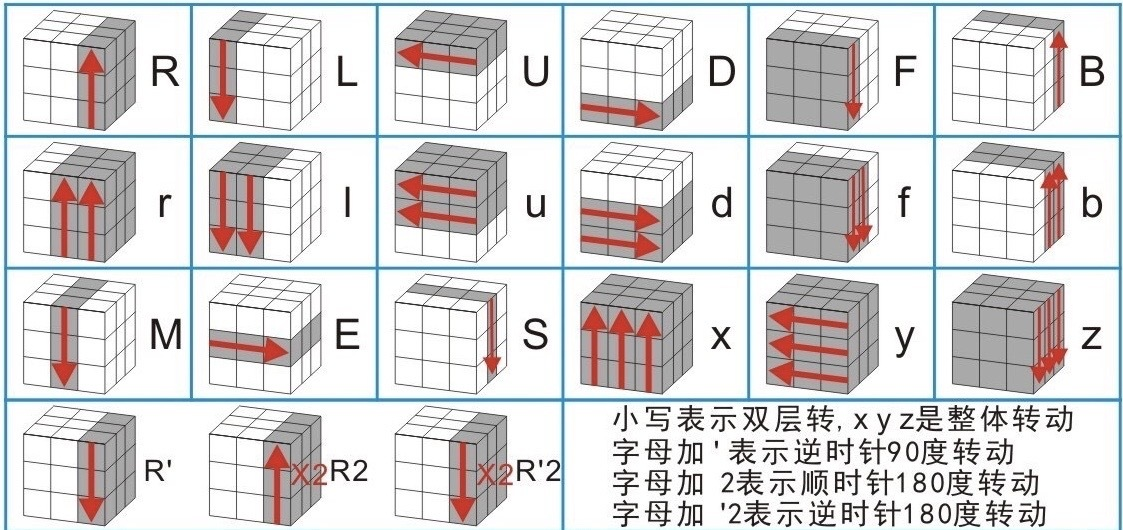
\includegraphics[scale=.27]{./rotate.jpg}
    \caption{转动符号系统说明}
    \label{转动符号系统说明}
\end{figure}
\end{frame} 

\begin{frame}
    \begin{figure}[!htb]
        \centering
        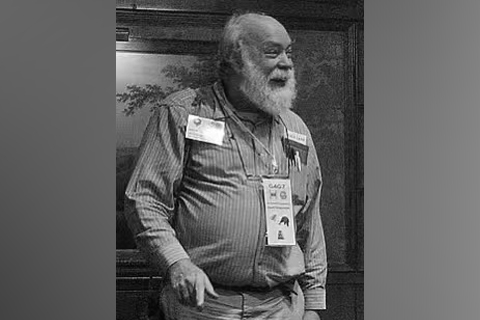
\includegraphics[scale=.6]{./xms.jpg}
        \caption{Singmaster}
        \label{Singmaster}
    \end{figure}
\end{frame} 




% \section{几个问题}
\begin{frame}{几个问题}
\begin{itemize}
    \item 魔方处于什么状态可以被还原 ?
    \item 魔方有多少种状态 ?
    \item {\bf 怎么定义魔方的数学结构} ? \lr  这样的数学结构有什么性质 ?
\end{itemize}
\end{frame} 


\begin{frame}
实际上魔方{\bf 可还原状态}约有 $8!\times 12!\times 2^{10}\times 3^7 \approx 4.3\times 10^{19}$,
但是如果我们从不严谨的角度来看待这个问题,我们可以从如下的角度思考:
魔方的种类数计算公式, 12个棱块,8个角块;每个棱块2个朝向,每一个角块3个朝向;
同时有一个限制 \lr 个棱块,角块是无法单独翻转[6]的,于是计算公式如下
\begin{align*}
     N = \frac{8!\times 12!\times 2^{12}\times 3^8}{12} = 43252003274489856000
\end{align*}
\end{frame} 

\begin{frame}
    \kaishu
    \noindent\rule{1\linewidth}{2pt}

    1. 如果不考虑朝向,只考虑色块的位置,那么我们拧魔方的操作实际上是全体色块位置的一个 {\bf 偶置换[2]}

    2. 色块朝向是一个2(3)阶循环群 $G_e = \langle g \rangle, G_v = \langle g' \rangle$
\end{frame} 

\begin{frame}{魔方第一基本定理}
一个魔方的状态由以下的条件唯一确定:
\begin{multicols}{2}
    \begin{itemize}
        \item 每一个棱块的位置
        \item 每一个棱块的朝向
        \item 每一个角块的位置
        \item 每一个角块的朝向
    \end{itemize}
\end{multicols}

看起来似乎就是一句废话 $\sim\sim\sim$
\end{frame} 

\begin{frame}
这是我们的一些规定:每一个棱色块的正方向为魔方处于初始状态时这个位置棱块的正面色
(自己选取,一般使用还原魔方的自然定义)的朝向.

下面我们为了方便,我们对魔方的全体棱块与角块进行排序(随意排序均可),从而确定每一个色块的方向是
$G_{e}^{12}$(全体12个棱块的朝向的所有情况)或 $G_v^{8}$的几个分量。
\end{frame} 




\section{群定义}
\begin{frame}
    首先定义{\bf 魔方群} $G$,其中的乘法 $x\circ y$定义为: 先进行 $x$ 操作,然后再进行 $y$ 操作,
我们称这个群 $G$ 为魔方群(Rubik's Group).
\begin{align}
    G = \langle R, L, F, B, U, D\rangle
\end{align}

定义群 $H$ 为将魔方从初始状态变换到任意状态(包括可还原和不可还原)的全体,
其中的乘法 $x\circ y$定义为: 先进行 $x$ 操作,然后再进行 $y$ 操作.
\end{frame} 

\begin{frame}
令 $S_E(=S_{12})$ 表示棱块的位置变换全体, $S_v(=S_8)$表示角块的位置变换全体,
其中的乘法 $x\circ y$定义为: 先进行 $x$ 操作,然后再进行 $y$ 操作.

为了把(操作) $g\in H$ 对色块的作用{\bf 提取}出来,我们需要使用到同态的概念.
\end{frame} 
\begin{frame}
我们建立了如下两个群同态 $\sigma,\; \rho$
\begin{align}
    \sigma: H \lr S_E
    \hspace*{4em}
    \rho: H \lr S_v   
\end{align}

$\sigma$ 将魔方的变换 $g\in H$ 映射到这个变换对全体{\bf 棱块}的位置变换,而
$\rho$ 将对魔方的全体变换 $g\in H$ 映射到这个变换对全体{\bf 角块}的位置变换.

\vspace*{4em}
\noindent\rule{1\linewidth}{2pt}
{
    \kaishu
    比如我做一个 $R$,本质上对于 $S_E$ 来说就是一个四轮换。
}
\end{frame} 

\begin{frame}
然后我们再定义两个映射 
\begin{align}
    \begin{aligned}
        w: H & \lr G_e^{12} \\
        g & \sr w(g) 
    \end{aligned}
    \hspace*{4em}
    \begin{aligned}
        z: H & \lr G_v^{8} \\
        g & \sr z(g) 
    \end{aligned}
\end{align}

其中 $w(g)$ 的第 $i$ 个分量表示初始状态下的第 $i$ 个棱块在经过变换 $g$ 后改变的方向,
也可以认为就是初始状态下位于第 $i$ 个位置的棱块经过变换 $g$ 后改变的方向
\end{frame} 

\begin{frame}
    比如 $H$ 中的元 $F$ 作用在 $S_e$ 后会产生如下的效果:
\begin{center}
    \begin{tabular}{p{.4\linewidth}p{.4\linewidth}}
        \toprule
        $g$ & $w(g)$\\
        \hline
        $F$ & $\{1,0,0,0,0,1,0,0,0,0,0\}$\\
        \bottomrule
    \end{tabular}
\end{center}
\end{frame} 

\begin{frame}
    实际上这个已经与群的外半直积类似了,可以向这个方向思考解决问题。
我们这里采用 {\bf 降群法}(Schreire-Sims-Minktwits 算法)来处理。
这个算法除了解决魔方问题,还可以解决其他类似问题,其核心就是下面证明部分要讲的内容。

\vspace*{6em}
\noindent\rule{1\linewidth}{2pt}

{
    \kaishu 
    如果有两个群 $N$ 和 $H$,以及群同态 $\psi:H \lr Aut(N)$, 则定义 $N$ 与 $H$
的外半直积 $N\rtimes H$ 成为一个群。
}
\end{frame} 




\section{引理}
\begin{frame}
    现在我们考虑一个初始状态的魔方,任取一个操作,重复有限次之后,必然会回到初始状态。
\begin{lemma}[有限群]
	$\forall P \in G,\exists k \in \mathbf{N},\mbox{使得}\; P^k = 1\mbox{且}\; P^{i} \neq 1,i = 1,2,\ldots,k-1$	
\end{lemma}
\begin{proof}
	对任取的$P$,考虑$\langle P\rangle = \{P^n|n=0,1,2,\cdots \}$.注意到$\left|G\right| < \infty$,因此$\langle P\rangle$必是有限群.
	由于$\langle P\rangle$是$G$的子群,我们熟知有限群的子群必然是有限的,因此原命题成立.
\end{proof}
\end{frame} 


\begin{frame}
为了使得迭代过程能够进行,我们还须使用如下的引理
\begin{lemma}[Schreier Subgroup Lemma]
    {
        \itshape
        Let $G$ be a group with a set of  generators $S$, Let $H$ be a subgroup 
        of $G$, and let $R$ be the set of coset representatives of 
        $H$ in $G$. For any $g\in G$, let $[g]$ denote the element 
        of $R$ that represents the coset $gH$,{\rm i.e.} 
        $[g] = gH$, and $[g]$ lies in $R$.
        
        Then $H$ is generated by the set $\{[sr]^{-1}(sr)\big|r\in R, s\in S \}$
    }
\end{lemma}

\noindent\rule{1\linewidth}{2pt}
    
{\kaishu Schreier子群引理说,给我们$G_i$的Generator集合,以及$G_{i+1}$的陪集集合,
我就可以生成$G_{i+1}$的Generator集合}
\end{frame} 

\begin{frame}
对于循环群的生成元我们有如下的引理,设有$n$个不交循环群生成元,
$\sigma_1,\sigma_2,\ldots,\sigma_n$,其阶数分别为$k_1,k_2,\ldots,k_n$.则有
    
\vspace*{1em}
\begin{lemma}[循环群的阶]
    $Order\{\sigma_1\sigma_2\ldots\sigma_n \} = {LCM}(k_1,k_2,\ldots,k_n)$.
\end{lemma}

\vspace*{6em}
\noindent\rule{1\linewidth}{2pt}

{
    \kaishu 
    $LCM$ 表示最小公倍数
}
\end{frame} 






\section{问题代数化}
\begin{frame}
魔方的还原问题用代数语言描述即为,给定一个$S_n$的子群$G$,以及$G$的生成集$S$,
\begin{align}
    S = \{U,D,L,R,F,B\}	
\end{align}

任意$g\in G$,求一个由$S$中元素构成的序列$\{x_1,x_2,\cdots,x_k \}$,
使得$g = x_1\circ x_2\circ \cdots\circ x_k$

根据前文可以知道,魔方的每个状态对应$A_{54}$中的一个元素,而每个元素均为$\{1,2,3,...,54\}$的一个全排列.
我们把面的全体记为$M$.
\end{frame} 

\begin{frame}
    任取$M$中元素$S = \{i_1, i_2,\cdots,i_{54}\}$,存在双射
\begin{align}
    \begin{aligned}
        F:G\bigg/Stab(G, S) &\longleftrightarrow Orbit(G,S)\\
        Stab(G, S)\circ g & \longleftrightarrow g\circ S
    \end{aligned}
\end{align}

% 这是因为两个有限集之间存在双射当且仅当基数相同.
\end{frame} 

\begin{frame}
\lr 怎么理解这个双射\; ?? 

{   
    \kaishu
    $Stab(G,S)$ 中的操作均无法转动 $S$,现在我们来看它的陪集
    $g\circ Stab(G,S)$, 因$Stab(G,S)$无转动作用,故 $\forall x\in Stab(G,S),$
    $g\circ x$ 均会将 $S$ 旋转到相同的位置,即 $g$ 的位置.也就是说,
    $Stab(G,S)$的陪集 $g\circ Stab(G,S)$,与$S$能被旋转到位置,是一一对应的.

    而陪集完整覆盖魔方群$G$。所以$Stab(G,S)$的商
    同构于$S$的轨道($S$能到达的所有位置):$G/Stab(G,S) \longleftrightarrow Orbit(G,S)$。
}
\end{frame} 

\begin{frame}
    我们可以定义如下的{\bf 稳定链}
\begin{align}
	G & \supset Stab(G,x_1) \supset Stab\left((Stab(G,x_1)), x_2\right) \cdots \notag\\
	  & \supset Stab\left(Stab\left(Stab(G, x_1),x_2\right),x_3\right)\notag \\
	  & \supset \cdots \supset \{e\}	
\end{align}

由于 $Stab(Stab(G, x_1), x_2) = Stab(G, \{x_1, x_2\})$,令$G_i = Stab(G,\{x_1,\ldots,x_i\})$,
那么上式可以简化为
\begin{align}
	G_0 \supset G_1 \supset \cdots \supset G_n=\{e\}
\end{align}
\end{frame} 

\begin{frame}{一次分解}
    根据定义我们有 $Stab(G_i, x_{i+1}) = G_{i+1}$, 我们使用如下的
方法来对 $g\in G$进行分解:
首先对于 $g_0 \in G$,我们先对其作一个初步分解: $g_0 = h_0\circ h_1\cdots h_{n-1}$,其中
$h_i \in G_i$.
\end{frame} 

\begin{frame}
    算法流程如下,$\forall g_i \in  G , \mbox{有} g_i\circ x_{i+1} \in Orbit(G, x_{i+1})$
\begin{align*}
	F^{-1}(g_i\circ x_{i+1}) 
	& = h_i \circ Stab(G_i, x_{i+1}) = h_i\circ G_{i+1}\\
	& \Longrightarrow g_i\circ x_{i+1} = F(h_i\circ G_{i+1}) \\
	& \Longrightarrow g_i \circ h_i^{-1}x_{i+1} = x_{i+1} \\
	& \Longrightarrow g_i h_i^{-1} \in G_{i+1}
\end{align*}

这意味通过$G_i$中的一个元素,我们可以求出$G_{i+1}$中的一个元素.
\end{frame} 

\begin{frame}
    于是给定 $g_0\in G$,我们可以找到满足以下条件的序列:
    $\{h_0, h_1,\cdots,h_{n-1}\}$ 使得
\begin{align}
	g_0h_0^{-1} \in G_1(g_0h_0^{-1}) h_1^{-1} 
	\in G_2\cdots g_0 h_0^{-1}h_2^{-1}\cdots h_{n-1}^{-1}
	\in G_n = \{e\}
\end{align}

这意味着$g_0 h_0^{-1}h_2^{-1}\cdots h_{n-1}^{-1} = e$,也即
\[
	g_0 = h_{n-1}h_{n-2}\ldots h_0
\]
\end{frame} 

\begin{frame}{二次分解}
    对于上式中的每一个 $h_i$,我们利用 {\bf Schreier's subgroup Lemma} 进行计算.
对于 $G_i\supset G_{i+1}$, 以及 $G_i$的生成子集 $S_i$, 我们可以利用
$G_i,S_{i+1}$ 计算得到 $Orbit(G_{i}, x_{i+1})$及一组 $G_i\big/G_{i+1}$
中的用$S_i$中元素或者其逆的乘积表示的表示元。设这组元表示为
\begin{align}
    U = \{u_1,u_2,\cdots, u\big|Orbit(G_i, x_{i+1})\}
\end{align}
\end{frame} 

\begin{frame}
    最终,我们将得到期望的所有 $Orbit(G_i, x_{i+1})$,然后利用Minktwits算法,
我们计算一组新的表示元(虽然在上述算法过程中,能得到一组表示元,
但那组表示元可能每个的 字长比较长,所以不能直接用)。

我们可以根据我们建立的双射 $F$ 来求出 $S$中对应的元素 $x_k$,
从而就完成了$g\in G$的分解,也就求解出了魔方。
\end{frame} 




\newcommand{\scale}[2]{%
    \scalebox{#1}[#1]{#2}}
\section{结语}
\begin{frame}[plain]
    \centering
    \scale{6}{Thank You}

    \vspace*{7em}
    \noindent\rule{.9\linewidth}{2pt}

    汇报小组:管虹安\quad 丁宗平\quad 覃俊杰\quad 张晓鹏
\end{frame} 

\end{document}